\documentclass[a4paper,12pt]{article}
\usepackage[english,activeacute]{babel}
\usepackage[ansinew]{inputenc}
\usepackage[T1]{fontenc}
\usepackage{amsmath,amsfonts,amssymb}
\usepackage{graphicx}
\usepackage{titlesec}
\usepackage{longtable}
\usepackage{dsfont}
\usepackage{wrapfig}
\usepackage{hyperref}
\usepackage{cancel}
\usepackage{epigraph}
\usepackage{appendix}
\usepackage{marvosym}
\usepackage{enumerate} %For enumerating with letters with option [a)]
\usepackage{fancyvrb} %To reduce font size in verbatim environment
\usepackage{epstopdf}
\usepackage[flushleft]{threeparttable}
\usepackage{natbib}
\usepackage{subfig}
%\usepackage{subcaption}
\usepackage{etoolbox}
\usepackage{array}
\usepackage{booktabs}
\usepackage[super]{nth}
\usepackage{breqn} %Breaks equations automatically
\usepackage{float}

\setlength\epigraphwidth{10cm}
\setlength\epigraphrule{0pt}
\newcolumntype{P}[1]{>{\centering\arraybackslash}p{#1}}


\newtheorem{definition}{Definition}
\newtheorem{proposition}{Proposition}
\newtheorem{theorem}{Theorem}
\newtheorem{corollary}{Corollary}

% === To embed exercises within the notes === %
\newtheorem{exercise}{Exercise}

\newcommand{\ts}{\textsuperscript}
\newcommand{\source}[1]{\caption*{\tiny Source: {#1}} }
\DeclareMathOperator{\sgn}{sgn}

\usepackage[left=2cm,right=2cm,top=2cm,bottom=2cm]{geometry}


\title{\textbf{QED Macroeconomics III: Problem Set Matlab 1}}

\author{Rafael Serrano Quintero
\thanks{Department of Fundamentos del An{\'a}lisis Econ{\'o}mico, Universidad de Alicante. Email: \texttt{r.serrano@ua.es}} \\
Universidad de Alicante \\}
\date{}


\begin{document}
\maketitle

\textbf{The due date for this Problem Set is Tuesday \nth{17} April 2018 before the class.} 

\textit{Please, try to send it earlier so I can take a look at your codes before the class.}

\begin{exercise}
Write one function \texttt{sumprodab} that produce as output the sum and the product of two numbers $a$ and $b$. The output \textbf{must} be of the form:
	\[
	\text{\textit{``The sum of \phantom{___} and \phantom{___} is equal to \phantom{___}''}}
	\]	
	\[
	\text{\textit{``The product of \phantom{___} and \phantom{___} is equal to \phantom{___}''}} 
	\]
	
	\underline{Hint:} check strings and \texttt{num2str()} command.
\end{exercise}

\begin{exercise}
Solve the following systems of equations:
\begin{enumerate}[a)]
	\item 	
	\begin{alignat*}{7}
	2x_1 & {}+{} & x_2  & {}-{} & x_3 & {}={}  & -1 \\
	2x_1 & {}-{} & x_2  & {}+{} & 3x_3  & {}={} &  -2 \\
	3x_1 & {}-{} & 2x_2 & {}={} & 1 &
	\end{alignat*}
	
	\item 
	\begin{alignat*}{7}
	2x_1  & {}+{} & 3x_2 & {}={} & 8 \\
	3x_1  & {}-{} & x_2  & {}={} & -2 \\
	-3x_1 & {}+{} & x_2  & {}+{} & x_3 & {}={} & 0
	\end{alignat*}
	
\end{enumerate}
\end{exercise}


\begin{exercise}
Simulate an AR(1) process. To do so, construct a function that takes as arguments the initial condition of the AR(1), the autoregressive parameter, the length of the simulation, and the variance of the error term. Recall an AR(1) takes the form:

\[
y_{t+1} = \rho y_t + \varepsilon_{t} \ ; \ \varepsilon\thicksim \mathcal{N}(0, \sigma^2)
\]

\textit{\underline{Hint:} loops might be useful in these cases. Check} \texttt{randn} \textit{function to generate random numbers.}

The function should return the vector $y_t$ and a plot of the AR(1). To test the function, choose $T = 100$, $\rho = 0.95$, $y_0 = 0$, and $\sigma = 0.5$;

\end{exercise}


\begin{exercise}
Plot the convergence of two infinite series. Suppose first we have the geometric series:

\[
G = \sum_{k=0}^{\infty} p^k = \frac{1}{1-p}
\]

Assume a value for $p =  0.99$ and $k$ should be all integers. First, calculate each term of the series in a vector. Then compute the cumulative sum of the vector that contains each term of the series. The cumulative sum of a vector is just another vector of the same size in which each element equals the sum of all the elements to the left of it in the original vector (\textit{\underline{Hint:} check} \texttt{cumsum}). Use the first $1000$ integers to compute the series.

Repeat the same but for the $p-$Series:

\[
P = \sum_{n=1}^{\infty} \frac{1}{n^p} = \frac{\pi^2}{6}
\]

Let $p=2$ and $n$ be the first $200$ integers.

Plot the convergence against the $k$ and $n$ integers in each of the series. The result should look something like Figure \ref{fig_series}.

\begin{figure}[htbp]
\centering
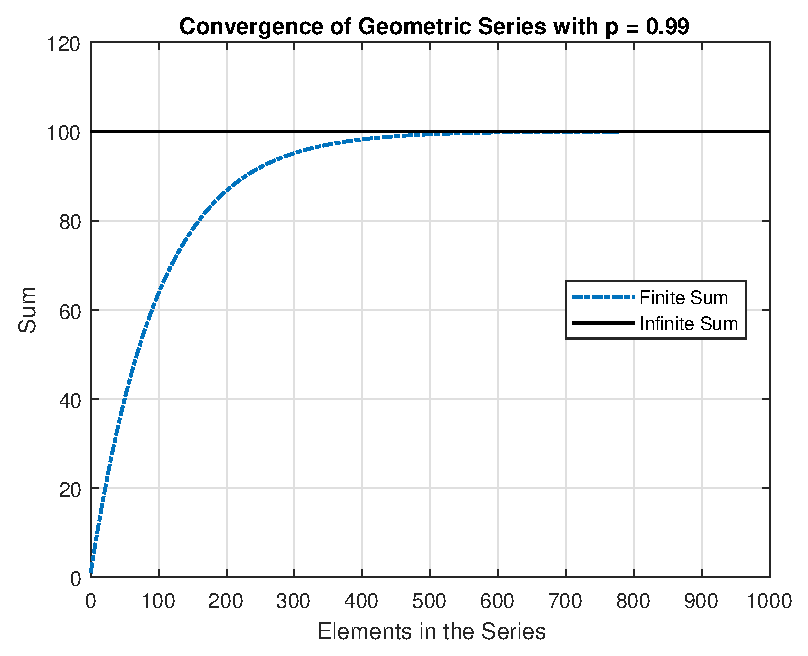
\includegraphics[width = 0.45\textwidth]{geoseries.eps}
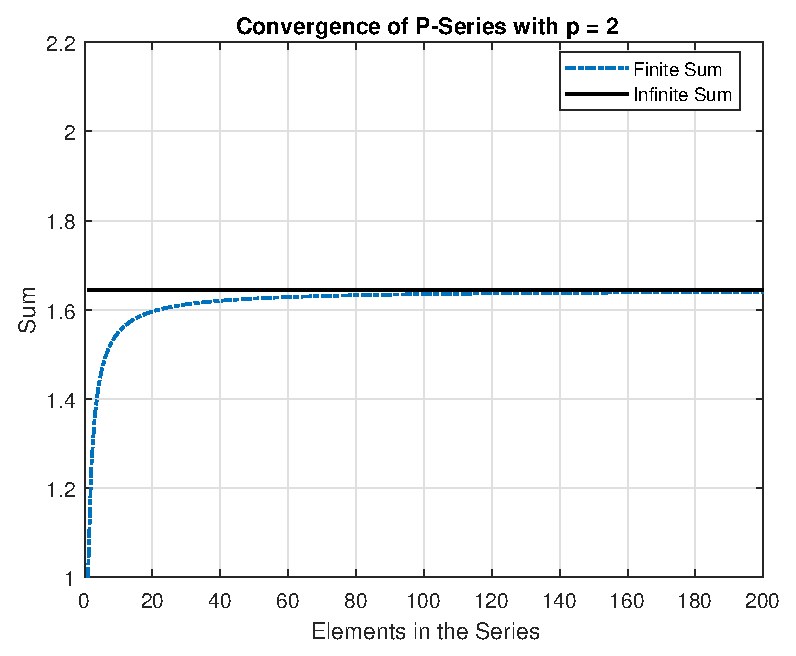
\includegraphics[width = 0.45\textwidth]{pseries.eps}
\caption{Convergence of the Series}
\label{fig_series}
\end{figure}
\end{exercise}

\begin{exercise}
Try to create a function that returns the first $n$ terms of the Fibonacci sequence. This sequence is characterized by the fact that each successive element of the sequence is the sum of its two predecessors (after the first two terms). So the sequence starts as:

\[
0, 1, 1, 2, 3, 5, 8, 13, 21, 34, 55, 89, 144,...
\]

So, generally, we can compute recursively element $n$ of the sequence as $F_n = F_{n-1}+F_{n-2}$ given $F_0 = 0$ and $F_1 = 1$. Within the function, set the first two elements and then, recursively, compute the first $n$ terms.
\end{exercise}

\begin{exercise}
Create a function \texttt{my_polynomial} that evaluates a polynomial of degree $n$ given its coefficients. That is, let a polynomial $p(x)$ be defined as:
	
	\[
	p(x) = \sum^n_{i=1}a_i x^{i-1}
	\]	
	
	You should write a function that takes as inputs coefficients $a_i$ and a value for $x$, then compute the value of the polynomial at that point $x$ given the coefficients. Furthermore, the function should also return the coefficients of the derivative of the polynomial.
	
	\textit{\underline{Hint:} for the derivative, note how is the general form of the derivative of these kind of polynomials, do not try to compute the derivative using Matlab but find a general form for it and write it in the function yourself.}
\end{exercise}

\begin{exercise}
Solve Solow's growth model. Write a function \texttt{solow} that takes as inputs the parameters of the model, solves for the series of capital in efficiency units, and plots the convergence to the steady state. If you feel like trying, plot a Solow diagram as well.
	
	\textbf{Solow's growth model:} Let the output be produced by a constant returns to scale (homogeneous of degree 1) Cobb-Douglas production function where $Y_t$ denotes output, $A_t$ denotes technology level, $K_t$ denotes capital stock, $L_t$ population (labour).
	
	\[
	Y_t = K_t^{\alpha} \left(A_t L_t\right)^{1-\alpha}
	\] 	
	
	Capital accumulates with a fixed proportion of output $(s)$ dedicated to investment minus the depreciated capital at a constant rate $\delta$.
	
	\[
	K_{t+1}	= sY_t +(1-\delta) K_t
	\]
	
	Technology and population grow at exogenous constant rates $A_t = A_0 (1+g)^t$ and $L_t = L_0 (1+n)^t$.	Let us do the following transformation, variables in lowercase letters are defined as $x_t = \frac{X_t}{A_t L_t}$. Then we can approximate the law of motion for capital as:
	
	 \begin{equation}
	 k_{t+1} \approx s k_t^{\alpha} + (1-n-g-\delta)k_t
	\label{klawofmotion}
	 \end{equation}
	
	 
	 The steady state is defined as $k^* = \left(\frac{s}{n+g+\delta}\right)^{\frac{1}{1-\alpha}}$.
	 
	 \textbf{Back to the code:} this is the discrete time version of the model and Equation \eqref{klawofmotion} is an approximation that becomes arbitrarily good as it converges to the steady state and, in continuous time, it is exact.
	 
	 Use Equation \eqref{klawofmotion} to show the convergence of capital to the steady state. Use the production function to show also the evolution of output over time. The logic of the code should follow something like:
	 \begin{itemize}
	 	\item The inputs of the function should be all parameters of the model, initial capital, and the length of the simulation $(A_0, L_0, n, \delta, g, s, \alpha, k_0, T)$.
	 	\item Compute the value of the steady state and define a vector of length $T$ with this value. (\textit{\underline{Hint:} check function} \texttt{ones()}).
	 	\item Compute recursively the capital series using Equation \eqref{klawofmotion}.
	 	\item Compute output using the production function with the capital series computed before (note this is capital in intensive form).
	 	\item Plot the convergence to the steady state and the series for output in a different figure. \underline{Hint:} check command \texttt{figure} to display more than one figure with the same script.
	 \end{itemize}
	 Test your function with the following values for the parameters:
	\[
	 A_0 = L_0 = 1, n = 0.01, \delta = 0.15, g = 0.02, s = 0.35, \alpha = 1/3, k_0 = 0.25, T = 60
	 \]
\end{exercise}
\end{document}